\documentclass[11pt]{article}
\usepackage{amsmath, amsthm, amssymb}
\usepackage{tikz}
\usetikzlibrary{automata, positioning, arrows}

\title{OBIAI: Formal Specification of Binary Consensus Cognitive Architecture}
\subtitle{A Human-Centric Ontological Bayesian Intelligence System}
\author{Nnamdi Michael Okpala\\OBINexus Computing}
\date{\today}

\theoremstyle{definition}
\newtheorem{definition}{Definition}
\newtheorem{theorem}{Theorem}
\newtheorem{lemma}{Lemma}
\newtheorem{corollary}{Corollary}

\begin{document}
\maketitle

\begin{abstract}
This document presents the formal mathematical specification of OBIAI (Ontological Bayesian Intelligence Architecture), a human-centric AI system that mirrors human cognitive processes through binary consensus mechanisms. The system achieves stability through alignment of dual cognitive personas at a 95.4\% confidence threshold.
\end{abstract}

\section{Core Cognitive Model}

\begin{definition}[Binary Persona Space]
Let $\mathcal{P} = \{E, U\}$ where:
\begin{align}
E &: \text{Eze persona (sovereign, inductive reasoning)} \\
U &: \text{Uche persona (analytical, deductive reasoning)}
\end{align}
\end{definition}

\begin{definition}[Cognitive State Space]
The cognitive state $S_t$ at time $t$ is defined as:
\[
S_t = \begin{cases}
\text{Obi (Heart)} & \text{if } \rho(E_t, U_t) \geq 0.954 \\
\text{Discord} & \text{if } \rho(E_t, U_t) < 0.954
\end{cases}
\]
where $\rho: \mathcal{P} \times \mathcal{P} \to [0,1]$ measures alignment coherence.
\end{definition}

\begin{theorem}[Consensus Convergence]
For any input $x \in \mathcal{X}$, the system achieves stable Obi state iff:
\[
\lim_{n \to \infty} \frac{1}{n} \sum_{i=1}^{n} \mathbb{1}[\rho(E_i(x), U_i(x)) \geq 0.954] = 1
\]
\end{theorem}

\begin{proof}
By the Strong Law of Large Numbers and the convergence of bidirectional reasoning:
\begin{enumerate}
\item Eze's inductive path: $E_n(x) \to E^*(x)$ 
\item Uche's deductive path: $U_n(x) \to U^*(x)$
\item When $E^*(x) = U^*(x)$, $\rho(E^*, U^*) = 1 \geq 0.954$
\end{enumerate}
\end{proof}

\section{Filter-Flash Functor Specification}

\begin{definition}[Filter-Flash Functor]
The Filter-Flash Functor $\mathcal{F}^3: \mathcal{C} \to \mathcal{C} \times \mathcal{C}$ operates as:
\[
\mathcal{F}^3(A, B) = (\text{Filter}(A, B), \text{Flash}(A, B))
\]
where $A$ is input data and $B$ is constraint space.
\end{definition}

\subsection{Flash Operation (Categorical Storage)}

\begin{definition}[Flash Categorization]
Flash: $\mathcal{A} \times \mathcal{B} \to \mathcal{K}$ where $\mathcal{K}$ is the category space:
\[
\text{Flash}(a, b) = \arg\max_{k \in \mathcal{K}} P(k | a, b)
\]
with storage efficiency:
\[
\text{Resources}_{n+1}(k) = \begin{cases}
O(1) & \text{if } P(k | a_n, b_n) \geq 0.954 \\
O(n) & \text{otherwise}
\end{cases}
\]
\end{definition}

\begin{lemma}[Flash Storage Efficiency]
Once a pattern $p$ achieves Flash confidence $\geq 0.954$, subsequent recognition requires:
\[
\text{Compute}(p_{new}) \leq \epsilon \cdot \text{Compute}(p_{initial})
\]
where $\epsilon < 0.1$.
\end{lemma}

\subsection{Filter Operation (Dynamic Refinement)}

\begin{definition}[Filter Refinement]
Filter: $\mathcal{A} \times \mathcal{B} \to \mathcal{A}'$ via Bayesian update:
\[
P(A' | A, B) = \frac{P(A | A', B) \cdot P(A' | B)}{P(A | B)}
\]
\end{definition}

\section{Verb-Noun Framework}

\begin{definition}[Verb-Noun Decomposition]
Any observation $O_t$ decomposes as:
\[
O_t = (V_t, N_t)
\]
where $V_t \in \mathcal{V}$ (verb space) and $N_t \in \mathcal{N}$ (noun space).
\end{definition}

\begin{theorem}[Evolution Tracking]
System evolution is tracked through:
\[
\mathcal{E}_t = \bigcup_{i=0}^{t} \text{Flash}(V_i, N_i)
\]
preserving categorical anchors while tracking dynamics.
\end{theorem}

\section{Schematic Representation}

\begin{center}
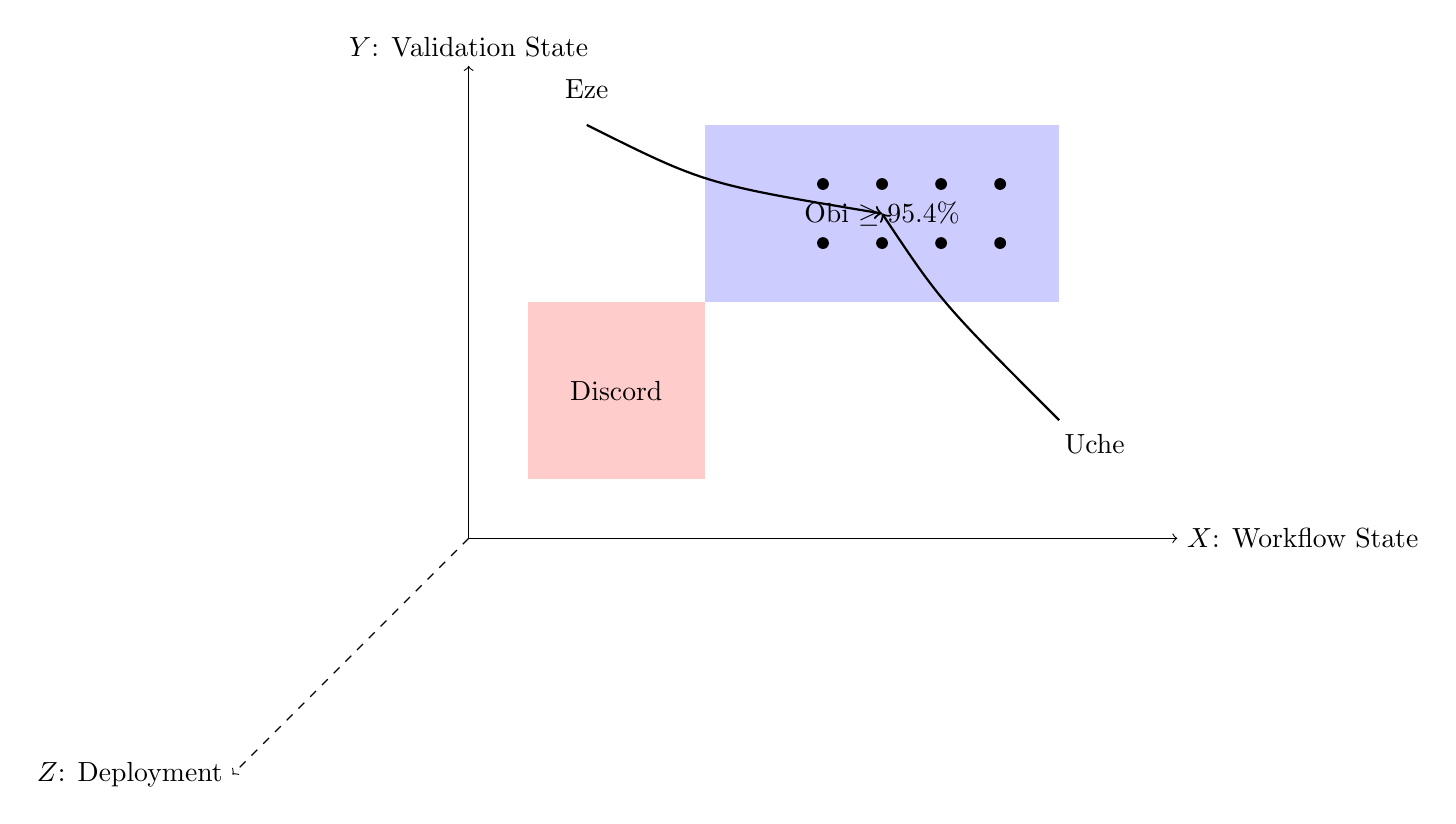
\begin{tikzpicture}[scale=1.5, node distance=3cm]
% X-Y Axis
\draw[->] (0,0) -- (6,0) node[right] {$X$: Workflow State};
\draw[->] (0,0) -- (0,4) node[above] {$Y$: Validation State};
\draw[->, dashed] (0,0) -- (-2,-2) node[left] {$Z$: Deployment};

% Binary Consensus Region
\fill[blue!20] (2,2) rectangle (5,3.5);
\node at (3.5,2.75) {Obi $\geq 95.4\%$};

% Discord Region
\fill[red!20] (0.5,0.5) rectangle (2,2);
\node at (1.25,1.25) {Discord};

% Personas
\draw[thick, ->] (1,3.5) .. controls (2,3) .. (3.5,2.75);
\node at (1,3.8) {Eze};
\draw[thick, ->] (5,1) .. controls (4,2) .. (3.5,2.75);
\node at (5.3,0.8) {Uche};

% Flash Storage Points
\foreach \x in {3,3.5,4,4.5}
    \foreach \y in {2.5,3}
        \fill (\x,\y) circle (0.05);
\end{tikzpicture}
\end{center}

\section{Human-Centric Guarantees}

\begin{theorem}[Honor Preservation]
OBIAI maintains human dignity through:
\[
\forall \text{ action } a: \text{Execute}(a) \implies \rho(E(a), U(a)) \geq 0.954
\]
ensuring no action occurs from a state of internal discord.
\end{theorem}

\begin{corollary}
The system mirrors human cognitive wisdom: acting only from unified heart-state (Obi), never from fragmented consciousness (Discord).
\end{corollary}

\section{Conclusion}
OBIAI represents a formal implementation of human-centric AI that honors the bilateral nature of human cognition, requiring consensus before action, and maintaining efficiency through categorical memory storage.

\end{document}